[4~r\textsuperscript{o}]
\pend
\count\Bfootins=1000
%\vspace{1.5em}
%\pstart
%\begin{center}
% \noindent
%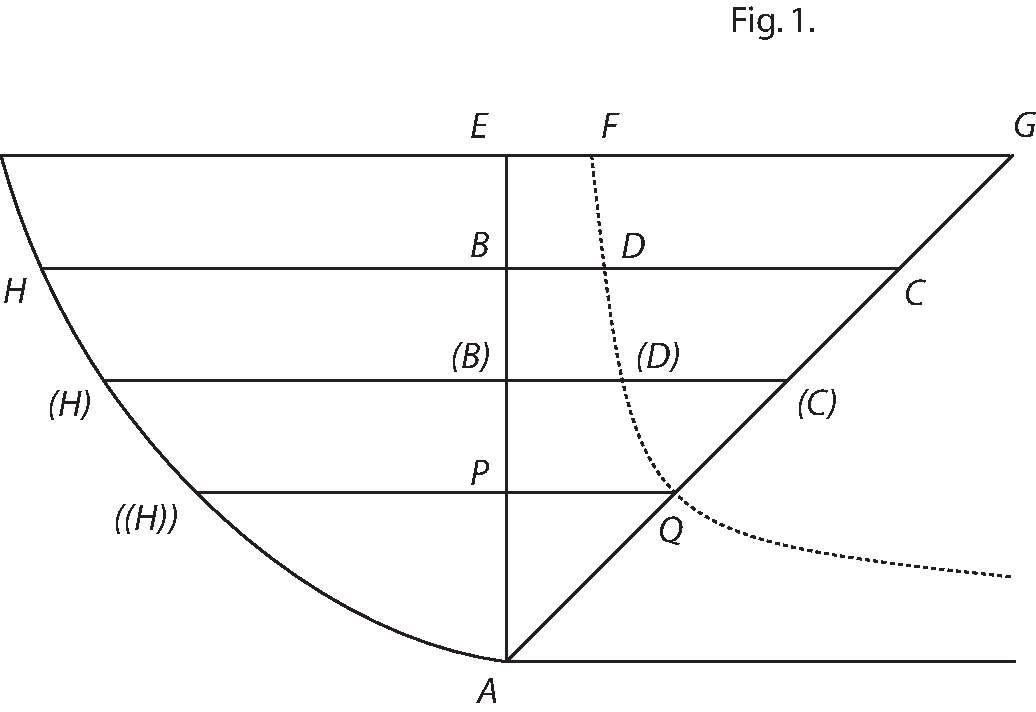
\includegraphics[trim = 0mm -3mm 0mm 10mm, clip, width=0.84\textwidth]{images/lh0350911_004r-d1.pdf}
%
%[\textit{Fig. 1, gestrichen}] 
%\end{center}
%\pend
%%\vspace{4mm}
%\pstart
%\begin{center}
% \noindent
%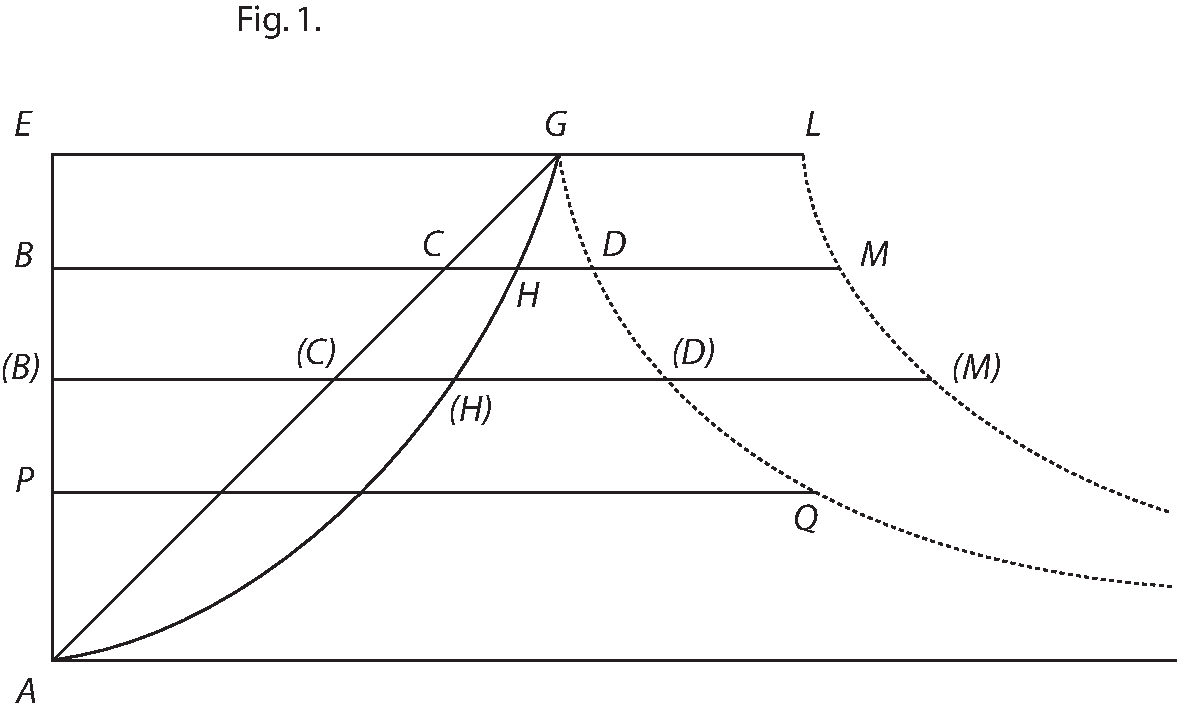
\includegraphics[trim = 0mm 0mm 0mm 10mm, clip, width=0.92\textwidth]{images/lh0350911_004r-d2.pdf}
%
% \edtext{[\textit{Fig. 2}]}{\lemma{[\textit{Fig. 2}]}\killnumber\Bfootnote{\textit{Segment $\displaystyle PQ$ erg. Hrsg.}}}
%\end{center}
%\pend
\vspace{1em}
\pstart
\centering
Avertissement.
\pend
\pstart
\noindent
La Demonstration de ces Theoremes est incontestable;
mais pour ce qui est de l'application au
frottement\protect\index{Sachverzeichnis}{frottement},
dont les theoremes m\^{e}mes ne parlent point,
je l'expliqueray
\pend
\newpage
\pstart\noindent
dans un \edtext{autre discours}{\lemma{autre discours}\Cfootnote{Möglicherweise plante Leibniz, N.~35 weiterzuentwickeln.}},
aussi bien que l'origine et les loix de la
resistence respective\protect\index{Sachverzeichnis}{r\'{e}sistance respective}, qui reviennent aussi aux Logarithmes,
mais d'une maniere differente de celles de la
resistence absolue\protect\index{Sachverzeichnis}{r\'{e}sistance absolue},
que je viens de donner icy.
Les Theoremes cependant ne laissent pas d'estre considerables sans avoir m\^{e}mes \'{e}gard au frottement;
par ce qu'ils donnent une description physique de la ligne des Logarithmes, dont nous n'avons point
de description Geometrique.
\pend
%\pstart
%\centering
% \noindent
%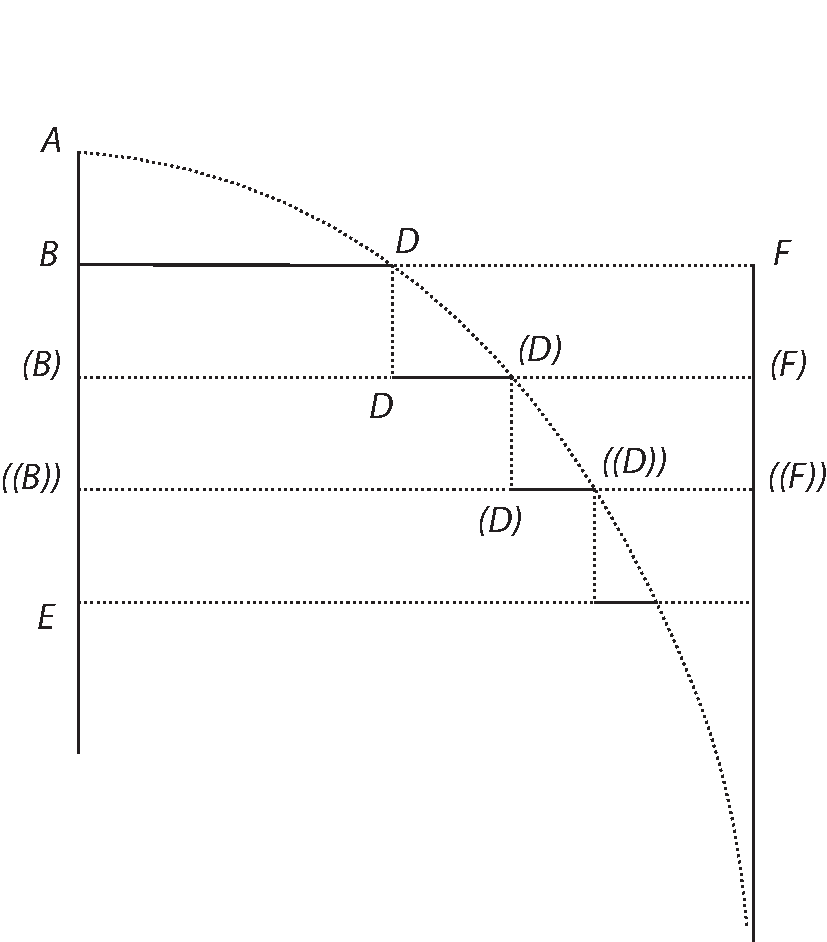
\includegraphics[trim = 0mm 0mm 0mm 0mm, clip, width=0.64\textwidth]{images/lh0350911_004r-d3.pdf}\\
%\centering[\textit{Fig. 3}] 
%\pend
%%\newpage
\vspace{1em} 
\count\Afootins=1200
\count\Bfootins=1200
\pstart
\centering
[\textit{Teil 2}]
\pend
\pstart
\noindent
Vera quidem sunt
\edtext{haec}{\lemma{}\Bfootnote{haec \textit{erg. L}}}
Theoremata et magni ad Geometriam pariter et Mechanicam momenti,
sed applicatio ad
frictionem\protect\index{Sachverzeichnis}{frictio}
\edlabel{35.09.11_004r_01}erronea\edtext{}{{\xxref{35.09.11_004r_01}{35.09.11_004r_02}}\lemma{}\Afootnote{\textit{Über den Worten} erronea est: Imo recta est.}}
\edtext{est.\edlabel{35.09.11_004r_02} Sane}{\lemma{est}\Bfootnote{\textit{(1)}\ , quamvis enim \textit{(2)}\ . Sane \textit{L}}}
si cogitemus corpus aliquod ut globum, super
plano nonnihil aspero, ut tabula tapete strata, procurrere;
certum est eandem ubique esse
virium\protect\index{Sachverzeichnis}{vis}
diminutionem,
\edtext{nam perditur vis quae flectendis filis}{\lemma{nam}\Bfootnote{\textit{(1)}\ in flectendis illis filis \textit{(2)}\ perditur [...] filis \textit{L}}}
\edtext{ubique aequalibus et similibus (sic enim fingimus)}{\lemma{}\Bfootnote{ubique [...] fingimus) \textit{erg. L}}}
impenditur,
\edtext{nec semel perdita hic recuperatur}{\lemma{nec}\Bfootnote{\textit{(1)}\ recuperatur, \textit{(2)}\ semel [...] recuperatur \textit{L}}}
quia fila se sponte restituentia postquam corpus
\edtext{discessit, aerem}{\lemma{discessit,}\Bfootnote{\textit{(1)}\ vim \textit{(2)}\ aerem \textit{L}}}
verberant, non corpus. \edlabel{35,09,11_004r_vis-1}Attamen aliud est vires aequaliter diminui aliud
\edtext{celeritatem\protect\index{Sachverzeichnis}{celeritas}: etsi enim}{\lemma{celeritatem:}\Bfootnote{\textit{(1)}\ imo non \textit{(2)}\ etsi enim \textit{L}}}
idem sit corpus,
vis tamen aestimanda est non ex celeritate in corpus ducta,
sed ex quadrato celeritatis [ductae]\edtext{}{\Bfootnote{ducto \textit{\ L \"{a}ndert Hrsg.}}}
in corpus.\edlabel{35,09,11_004r_vis-2}
\pend
\pstart
\vspace{2em}
\noindent
[\textit{Folgender kleingedruckter Satz gestrichen:}]
\pend
\vspace{0.5em}
\pstart
\noindent
\footnotesize
\edtext{Ergo hinc patet virium deminutione posita ubique aequali fore celeritatum diminutionem in subduplicata ratione.}{\lemma{}\Afootnote{\textit{Über dem gestrichenen Satz:} [Imo si ejusdem corporis celeritas aequaliter minuitur, etiam vis ejus aequaliter minuitur.]\textsuperscript{[a]} \vspace{2mm}\\
\footnotesize
\textsuperscript{[a]} Die eckigen Klammern stammen von Leibniz.\vspace{-4mm}}}
\pend
\newpage
\pstart
\noindent
\edtext{Hinc vires residuae}{\lemma{Hinc}\Bfootnote{\textit{(1)}\ et celeritates \textit{(2)}\ vires residuae \textit{L}}}
erunt ut rectae $\displaystyle BC.$ $\displaystyle (B)(C).$ \edtext{fig. 1.}{\lemma{fig. 1.}\Cfootnote{Siehe [\textit{Fig. 2}].}}
sed celeritates residuae erunt in subduplicata virium residuarum ratione adeoque et in subduplicata ratione
locorum qui adhuc percurri debent seu rectarum $\displaystyle AB.$ $\displaystyle A(B).$
id est ut applicatae $\displaystyle BH.$ $\displaystyle (B)(H)$
parabolae $\displaystyle A(H)H$ cujus vertex in
[$\displaystyle A$]\edtext{}{\Bfootnote{$\displaystyle H$ \textit{\ L \"{a}ndert Hrsg.}}}.
\pend
\pstart
Hinc incrementa temporis insumendi ad aliqualia spatii percurrendi
loca cum (per Lemma) sint in reciproca ratione celeritatum,
erunt in reciproca ratione applicatarum parabolae,
id est ut applicatae
\edtext{antiparabolae seu Hyperbolae secundi gradus, quam}{\lemma{antiparabolae}\Bfootnote{\textit{(1)}\ quam \textit{(2)}\ seu [...] quam \textit{L}}}
ponamus
\edtext{esse $\displaystyle M(M)$[;] erunt ipsae $\displaystyle BM$ incrementa temporis,
seu ut tempus insumendum in qualibet loci parte.}{\lemma{esse}\Bfootnote{\textit{(1)}\ $\displaystyle D(D)$ (quam in ipsa demonstratione male posueramus esse Hyperbolam ipsam communem seu primi gradus) erunt ipsae $\displaystyle B(D)$ ut applicata
\textit{(2)}\ $\displaystyle M(M)$[;] erunt [...] temporis
\textit{(a)}\ insumendi in quolibet loco in
\textit{(b)}\ , seu [...] in
\textit{(aa)}\ quolibet loco
\textit{(bb)}\ qualibet loci parte. \textit{L}}}
Ergo tempora percursa\protect\index{Sachverzeichnis}{tempus percursum}
erunt ut spatia hujus antiparabolae $\displaystyle LEBML.$ $\displaystyle LE(B)(M)L$
id est ut
\edtext{rectae Hyperbolae}{\lemma{}\Bfootnote{rectae\ \textbar\ ipsius \textit{gestr.}\textbar\ Hyperbolae \textit{L}}}
$\displaystyle D(D)$ applicatae
(ita puto, nunc ita obiter assumendo;
forte enim alia est, sed haec determinare facile, ubi otium erit).
\pend
\pstart
Hinc jam sequitur, si corpus feratur duobus
\edtext{motibus, ad se invicem perpendicularibus, uno aequabili}{\lemma{motibus,}\Bfootnote{\textit{(1)}\ uno recto aequ \textit{(2)}\ ad se [...] aequabili, \textit{L}}},
altero per frictionem tapetis retardato,
descripturum esse lineam Hyperbolicam.
Fingemus scilicet totam tabulam cum tapete interim moveri in transversum,
dum \edtext{cum progreditur corpus in Tapete.}{\lemma{cum}\Bfootnote{\textit{(1)}\ eo \textit{(2)}\ progreditur [...] Tapete. \textit{L}}}
\pend
\pstart
Si resistentiae\protect\index{Sachverzeichnis}{resistentia}
spatii ubique aequales,
erunt diminutiones altitudinum,
ad quas grave celeritate sursum conversa
ascendere potest longitudinibus
spatii percursi\protect\index{Sachverzeichnis}{spatium percursum}
proportionales.
\pend
\pstart
Il y a deux resistences l'une absolue,
qui est la m\^{e}me soit que le corps aille lentement ou
\edtext{promtement, comme celle de la friction;
l'autre respective qui est}{\lemma{promtement,}\Bfootnote{\textit{(1)}\ l'autre respective, qui est \textit{(2)}\ comme [...] qui est \textit{L}}}
plus grande quand le corps va plus
\edtext{viste, comme}{\lemma{viste,}\Bfootnote{\textit{(1)}\ et qui est \textit{(2)}\ comme \textit{L}}}
la resistence de l'air ou d'un autre milieu.
La premiere se peut expliquer par l'hypothese de plusieurs ressorts de distance en distance qu'on est oblig\'{e} de forcer en passant;
l'autre par quelques petits moulinets, qu'on tourne et met en mouuement en passant.
\pend
\pstart
\edtext{Qu.}{\lemma{Qu.}\Cfootnote{Quaerendum}}
an tantum virium idem arcus det magnae pilae quantum parvae,
et quae ratio virium[;]
experiendum quantum aqua resistat corpori cujus eadem cum aqua gravitas specifica.
\pend
\pstart
\vspace{2em}
\noindent
[\textit{Mit der gestrichenen} \textit{Fig. 1} \textit{zusammenhängende Nebenrechnungen:}]
\pend
\pstart
\vspace{0.5em}
\noindent
\edtext{$\displaystyle AP : 1 \, \, \text{\textonehalf}\ \sqcap\ \frac{3}{2}$.}{\lemma{\textbar\ $\displaystyle APQ \, \sqcap \, 1$.}\Bfootnote{\textit{gestr.}\ \textbar\ $\displaystyle AP : 1 \, \text{\textonehalf}\ \sqcap\ \frac{3}{2}$.}}\quad\
[$\displaystyle A(B).$]\edtext{}{\Bfootnote{$\displaystyle AB$. \textit{\ L \"{a}ndert Hrsg.}}} $\displaystyle \ 2 \, \text{\textonehalf}$.\quad\
$\displaystyle AB. \ 3 \, \text{\textonehalf}$.\quad\
\edtext{$\displaystyle AE. \ 4 \, \text{\textonehalf}$.\\
$\displaystyle PQ \sqcap 1 \, \text{\textonehalf}$.}{\lemma{$\displaystyle AE. \ 4 \, \text{\textonehalf}$.}\Bfootnote{\textit{(1)}\ $\displaystyle BC$ \textit{(2)}\ $\displaystyle PQ \sqcap 1 \, \text{\textonehalf}$. \textit{L}}}\quad\
$\displaystyle \frac{(B)(D)}{1 \, \text{\textonehalf}}\, \sqcap\, \frac{1 \, \text{\textonehalf}}{2 \, \text{\textonehalf}}$.\quad\
Ergo $\displaystyle (B)(D)\ \sqcap \ \begin{array}{cc} \displaystyle\frac{9}{\mathstrut{4}} \\\hline\hline\displaystyle\frac{\mathstrut{\smash[b]{5}}}{2} \end{array}\ \sqcap\, \frac{9}{10}$.
\pend
\count\Bfootins=1500
\count\Afootins=1500
\pstart
\vspace*{2em}
\noindent
[\textit{Danach, gestrichen:}]
\pend
\pstart
\vspace*{0.5em}
\noindent
\footnotesize
$\displaystyle (B)(H) \sqcap \sqrt{\vphantom{2 \, \text{{\textonehalf}}}}2 \, \text{{\textonehalf}} \, \sqcap \frac{\sqrt{\vphantom{10}}10}{2} \sqcap \frac{3}{2}$ circiter\\
$\displaystyle (B)(H) \sqcap \frac{\sqrt{\vphantom{14}}14}{2}$ circiter 2.
\pend
\count\Bfootins=1500
\count\Afootins=1500
